\chapter{Results}
 In the previous chapter, a simple feedforward network with two layers has been made. The responses of various convergent connections in such network to static and oscillating input are discussed in this section. The goal for this research study is to investigate how information transfer as infer from output firing rate can be modulate by level of synchronization in the input and which convergent connection rule has the highest output response to this input synchronization.

 First, we describe the unique activity map under various kind of input and various kind of convergent connection rules.  We then show the increase in output firing rate when feedforward connection strength increase and when the synchronization level in input increase. 
We demonstrate that in Uniform-Uniform convergent rule(UU) has highest response gain from static input to oscillating input when compare to other convergent rules.  
Finally, we reveal that the UU rule has highest number of induced spike gain and it is highly dependent on phase of input oscillation. The explanation on why the UU rule is most sensitive to synchronized input based on idea of temporal summation was also introduced. 

%
%
%%Response Function
%
%Figure 1. Network of different types of convergence 
%
%Figure 2. Firing rate increases for oscillating input
%
%Figure 3. Gain function of firing rate for oscillation is greatest in UU
%
%Figure 4. Gain function of induced post-synaptic spike for one pre-synaptic spike is highest in UU model
%
%Figure 5. Post-synaptic activity is most tuned for oscillation in UU model
%


% Add this Question and Hypothesis in the method part too
\section{The activity map of target layer shows unique response for each combination of convergent rules and input pattern}
 For each combination of input pattern and convergent rules, an activity matrix has been made by assigned each element as average firing rate of target layer at given convergent conditions ( $r_i$, $w_i$). Three convergent rules and three input levels multiply to nine cases of activity matrix as shown in figure ~\ref{fig:ActivityMatrix} 
The contour plot from this matrix build up the activity map for each condition(Figure~\ref{fig:ActivityMap}). In the activity map the lighter color mean the higher firing rate.  In all the cases, when convergent conditions increase the response increase. However, the rate of increasing are different in each case as that can be easily observed when the compare the same position of the map in all cases (red dot position; $r_i$ = 80, $w_i$ = 80 ). 


%Activity Matrix
\begin{figure}[!h]
	\centering
	\includegraphics[width=0.9\textwidth]{figures/Result_ActMatrix}
	\caption{The activity matrix shows response of a feedforward network under different condition. Row~: Convergent Rules; Gaussian-Gaussian(GG), Uniform-Uniform(UU), and Uniform-Exponential(UE) , Column ~: Input pattern; static, weak oscillation, and strong oscillation input.}
	\label{fig:ActivityMatrix}
\end{figure}

%Activity Map
\begin{figure}[!h]
	\centering
	\includegraphics[width=0.9\textwidth]{figures/Result_ActMap}
	\caption{The Activity Map that made from contour plot of activity matrix. Red dots shows the location of same convergent condition in each case but they have different response due to input pattern and convergent rules}
	\label{fig:ActivityMap}
\end{figure}


 To explore the role of each convergent condition parameter, the output firing rate were plot when one parameter is fixed.   If range of connection is fixed, the output  firing rate vs. weighting factor parameter were plot (Figure~\ref{fig:ObservedRfix}).  Likewise, if weight condition is fixed, the output  firing rate vs. range  parameter were plot (Figure~\ref{fig:ObservedWfix}). 
When observe the change in the output firing rate, we found that the strong oscillating input has highest response compare to the other input pattern in all cases.  


%Fix R , and fix W 
\begin{figure}[!h]
	\centering
	\includegraphics[width=1\textwidth]{figures/Result_fixRange}
	\caption{The observed response of network when range of connection fixed and varies weight}
	\label{fig:ObservedRfix}
\end{figure}

\begin{figure}[!h]
	\centering
	\includegraphics[width=1\textwidth]{figures/Result_fixWeight}
	\caption{The observed response of network when strength of connection (or weight) fixed and varies range of connection}
	\label{fig:ObservedWfix}
\end{figure}


\section{The feedforward network with strong oscillation input has highest output firing rate}
% The response function, average output firing rate over total feedforward 
 According to the observation in the previous part, it showed that the oscillating input gave higher response compare to the static input. Next, the general analysis is made for all the convergent conditions by look at relationship between output firing rate and total feedforward strength ( or total weight summation as introduced earlier).  From this plot (Figure ~\ref{fig:ResFun} ), it can clearly be seen that as total feedforward connection strengthen the output firing rate also increase.
 In addition, the firing rate in all convergent rules increases for oscillating input compare to the static input case. The slope of this plot can be considered as gain or average firing rate per unit feedforward strength.  Higher gain value means the feedforward network can transfer more spikes to output layer with the same connection strength to the lower gain value. The slope or gain from this response function were plot in Figure~\ref{fig:ResFunDiff}. From this plot, it can  clearly be  seen in all convergent rules that the strong oscillation  input has highest gain, then weak oscillation and static input respectively.  If we examine it further by look at the different in slope of strong oscillation input and that of static input of all convergent rules, we found that the Uniform-Uniform model has highest different in the gain value as in Figure~\ref{fig:ResFunDiff} B. 


\begin{figure}[!h]
	\centering
	\includegraphics[width=1\textwidth]{figures/Result_MeanFr_sumW}
	\caption{The response function (mean firing rate vs. total feedforward strength) of UU, GG, and UE from left to right. The firing rate increases when connection strengthens.}
	\label{fig:ResFun}
\end{figure}


\begin{figure}[!h]
	\centering
	\includegraphics[width=1\textwidth]{figures/Result_MeanFr_sumW_slope}
	\caption{Comparison of slope or gain. A. Firing rate increases for oscillating input. B. The UU model has highest different in firing rate between strong oscillation and static input.}
	\label{fig:ResFunDiff}
\end{figure}



\section{The Uniform-Uniform model has highest response gain from static input to oscillating input}
 In the previous section, the Uniform-Uniform model has highest oscillation-static different  in gain (average output firing rate over total feedforward connection strength ). Plus, it is known from the previous result that the feedforward network with oscillating input has higher response in target layer than the static input case.  
Next, in order to explore how much response in oscillating input increase from static input, the firing rate of each condition was scattered onto static input axis and oscillating input axis (Figure~\ref{fig:ResFunDiffOscS}). A linear fitting has been made for data from each of the convergent rules; Gaussian-Gaussian(GG),Uniform-Uniform(UU), and Uniform-Exponential(UE).   Then, the slope for each convergent rules population are determine and compared. The slope of this fitted line are defined as gain (output firing rate when given oscillating input over those when static input were given) and are plotted in Figure ~\ref{fig:ResFunDiffOscS_hp}. Since there are two kind of oscillation input, two comparisons can be made; weak oscillation vs static(WO-S), and strong oscillation vs static(SO-S). We found that in both comparison WO-S and SO-S, the Uniform-Uniform has highest gain from static to oscillation compare to the other convergent rules. The gain can infer to the sensitivity of each feedforward network to the synchronization level of input. 



\begin{figure}[!h]
	\centering
	\includegraphics[width=1\textwidth]{figures/Result_OscFR_StaticFR_Scatter}
	\caption{Comparing output firing rate of static input and oscillating input. WO-S, and SO-S are comparison between static input to weak oscillation and strong oscillation respectively.}
	\label{fig:ResFunDiffOscS}
\end{figure}


\begin{figure}[!h]
	\centering
	\includegraphics[width=0.5\textwidth]{figures/Result_OscFR_StaticFR_bar}
	\caption{The Uniform-Uniform model had the biggest gain from static to oscillation.}
	\label{fig:ResFunDiffOscS_hp}
\end{figure}

\section{The Uniform-Uniform model has highest number of induced spike gain on target layer from one spike in source layer}
 From previous result, the UU model  has highest response gain from static input to oscillating input. The further analysis was introduced to quantify the number of output spike that one input spike can made. This analysis starting with counting number of postsynaptic spikes in target layer that following each of the presynaptic spike in source layer when there exist connection between the layer. Then, normalised this count with total number of spikes to get the induced spikes plot. The area under the first peak of the curve cut by baseline activity is the yield induced spike.  Scattered these induced spike of static and oscillating input then we can investigated relationship between levels of synchronization in the input.The gain function then calculated from the ratio between induced spike from oscillation and induced spike from static (Figure ~\ref{fig:InduceCurve}. ). The average gain of each convergent rules are shown in Figure~\ref{fig:InduceBar}  with two types of oscillation-static comparison. The result shows that the number  of induced spikes in the Uniform -Uniform model is highest compare to the other two cases ( GG came in second, and UE had least gain). Plus, overall gains of induced spikes in SO-S case is higher than WO-S case which is expectable since the synchronization level in WO less than SO input. The highest gain in induced spike shows that the Uniform-Uniform convergent rules can produce more spike per one input spike. This result shows analysis in the cell level compare to the previous analysis that were looked upon properties in network level. 



\begin{figure}[!h]
	\centering
	\includegraphics[width=1\textwidth]{figures/Result_Induced_curve}
	\caption{Example plot for timing of the Induced target spike from a spike in source layer. The shade area, area under the first peak  to the baseline level, imply the number of total induced spikes.}
	\label{fig:InduceCurve}
\end{figure}

\begin{figure}[!h]
	\centering
	\includegraphics[width=0.4\textwidth]{figures/Result_Induced_bar}
	\caption{The number of induced spike gain from static to oscillation input. UU has highest gain in both level of oscillation. (T-test, $p < 0.05$)} % t-test
	\label{fig:InduceBar}
\end{figure}

 
\section{The output spikes in target layer of the Uniform-Uniform model depend on phase-lock to oscillation the most}
  All previous results showed that the strong oscillation has highest response compare to weak oscillation and static input. Also, the Uniform-Uniform convergent rules has the highest sensitivity to the change in static input to the oscillating input. 
Next question is how the output spikes related to the phase of the input pattern and how convergent rules behave differently on this phase-tuning. 
The output response - input phase relation has been made by count output spike timing in one period of input oscillation and sum up all the periods available in simulation.  The result can be shown in Figure~\ref{fig:PhaseCurve}. It appeared that the responses are phase lock to crest of oscillating input.
Since, we are interested in the gain or different of those value in oscillating input over static input, the plot for each convergent rules are normalised by its spike number in static input. From this curve, the full width half maximum (FWHM) were measure and the average values are plotted in bar graph (Figure~\ref{fig:PhaseBar}). The small width mean the response are sharply tune to the phase of oscillated input pattern. For Strong oscillation - static input comparison, the UE had stand out biggest width, the UU and GG has small width. Comparing  between the UU and GG model, they are significantly different with smaller width in UU. The WO-S comparison showed similar result but overall higher width in all cases. Therefore, this evidence suggest that the Uniform-Uniform model were tuned to phase of input oscillation the most.




\begin{figure}[!h]
	\centering
	\includegraphics[width=1\textwidth]{figures/Result_PhaseTune_curve}
	\caption{Spiking timing in one period of oscillation input pattern. Left, the example of the tuning plot . Right, the normalised spiking timing by that of static input and the width measurement, Full width at half maximum (FWHM).} 			\label{fig:PhaseCurve}
\end{figure}

\begin{figure}[!h]
	\centering
	\includegraphics[width=0.5\textwidth]{figures/Result_PhaseTune_bar}
	\caption{The UU convergent rule has the smallest width indicating the highest tuning to oscillation input compare to the GG and UE rules} 
	\label{fig:PhaseBar}
\end{figure}


\section{The Uniform-Uniform model has highest sensitivity to synchronized input because of its optimal distribution of weighting factor}
 The Uniform - Uniform convergent rules has the highest sensitivity to the level of synchronization in the input pattern as can be seen from the response gain from static to oscillating input, number of induced spike gain, and phase-lock to the oscillation.  The next question is to explain what happen in the Uniform-Uniform convergent rules  that make it sensitive to change in synchronization level in input.

\begin{figure}[!h]
	\centering
	\includegraphics[width=1\textwidth]{figures/WeightDistForOneCell}
	\caption{The distribution of weighting factors of convergent connections to a target cell} 
	\label{fig:WdistOne}
\end{figure}

 We has confirmed that the distribution of connection probability and connection strength are as we design in the methodology chapter(Figure~\ref{fig:WdistOne}). Adding on to that, the distribution of weighting factor of all cells in the target layer showed different distribution to that of single target cell due to stochastic in the system, as shown in Figure ~\ref{fig:WdistNN}). According to this distribution, the UE model has exponential distribution as expected. The UU model has normal-like distribution due to stochastic environment. The Gaussian-Gaussian model has almost flat distribution.  The Gaussian distribution has high weighting factor in center population and has lower weight value in boundary. However, due to the increase in area covering by the filter at the boundary where connection probability and weighting factor are low, the compensation for low connectivity effect occurred and bring up the  total number of low weight. As a result, the GG model has flat distribution (Figure~\ref{fig:WdistNN}).  When comparing cumulative sum of these distribution, the UU model clearly had narrow range of strength compare to conventional model like GG model.

\begin{figure}[!h]
	\centering
	\includegraphics[width=1\textwidth]{figures/WeightDistForNetwork}
	\caption{The distribution of weighting factors of all convergent connections to target layer. Small figure: Top the cumulative distribution function of weight distribution in all types. Bottom: The plot of 2D Gaussian filter shows increasing in ring area at boundary where the Gaussian value is low compare to the inner area that has high Gaussian value but it got limited space.} 
	\label{fig:WdistNN}
\end{figure}


\begin{figure}[!h]
	\centering
	\includegraphics[width=1\textwidth]{figures/WeightDistForSchematic}
	\caption{The schematic figure to employ idea of temporal summation \cite{magee1999dendritic}  to explain why the UU model has highest sensitivity to level of synchronization in input} 
	\label{fig:WdistSchematic}
\end{figure}



 The distribution in weighting factor or strength of a feedforward connection is key explanation on its sensitivity to synchronization level in the input.  We divided the group of weighting factor into three groups according to their range; low, middle, and high, then use it to explain feedforward connection characteristics and its response. In the case of high connection strength, spike from source cell can make spike in target layer. In case of low connection strength, it is hard to make spike cell from only single spike from source layer. However, at the middle range of connection strength, it is the range that the probability of making spike is not certain but depend on the pattern of input spikes and it can explained by idea of temporal summation in cell conductance (Figure~\ref{fig:WdistSchematic}). When there is no oscillation in the input, the spikes arrive the postsynaptic cell individually (not overlap or not too close to each other).  At this middle range of connection strength, the conductance of these single spikes cannot reach threshold of action potential, therefore it cannot produce spike in target cell.  If oscillating input were given at this same middle range of connection strength, however,  there are many spikes with short inter-spike-interval and many overlap spikes (because they are synchronized) which then their conductance sum up as in temporal summation idea and drive spike in target cell. The connection strength in the UU model clustered around middle range that is why the change in static and the strong oscilation in UU model is highest. 




%
%\section{Prof's suggestion}
%General Note : If you fix trial number to some n value --> explain why it is enough.  
%What are the meaning of these result in biological system
%\subsection{Proved your hypothesis}
%\paragraph{Hypothesis}  The brain (is it too big or too general?) need interlayer communication that optimized cost of the connection 
%which is achieved by the synchronized neural activity on source layer and statistical wiring diagram( with Gaussian distribution of connectivity and connection strength)
%
%\paragraph{Proving the Hypothesis}  Compare differences in these three cases of connection (Gaussian, uniformly random, random with negative exponential) of input variations
% ( osc  vs. no osc  ; varies F and Amp ) 
% The measurement can be  1) Fr ,  2) Spike Correlation, 3) Spike Pattern (Ex. M1 activity according to Input oscillating pattern, how is the phase affect the result etc )
%

%\begin{center}
%....................
%OLD
%....................
%\end{center}
%\section{ Answer to RQ1 : The computer simulation resemble experimental results of animal study}
%
%\subsection{ The single cell properties of computational model and the whole cell patch clamp recording shows the same behavior}
%
%Figure .1.1: Comparing the sample membrane potential trace of WT and KO during hyperpolarize current injection and depolarize current injection
%
%Figure .1.2: Comparing the number of bursting spikes and tonic spikes between the simulated cell and experimental data
%
%
%\subsection{  The cell population properties of computational model and the MUA cells recording shows the same behavior}
%
%Figure .1.3 : Comparison of mean and standard deviation of observed firing rate in cell population in computational model and experimental data
%
%
%\subsection{ Neuron activities during light-off period (no photoactivation)}
%
%Figure .1.4 The baseline activities of neural population during light-off period show no significant different between WT and KO
%
%
%\subsection{ Neuron activities during photoactivation}
%
%Figure .1.5 The delay and peak of rebound spiking activity of WT and KO are significantly different. The WT shows short rebounding period and higher peak of neural activities
%
%
%\subsection{ The coherence between VL and M1 layer shows that correlated neural activities after photoactivation ( the rebound bursting spikes) drives activity in M1}
%
%Figure~\ref{fig:sample} The coherence between VL’s MUA and M1’s LFP
%
%\begin{figure}
%	\centering
%	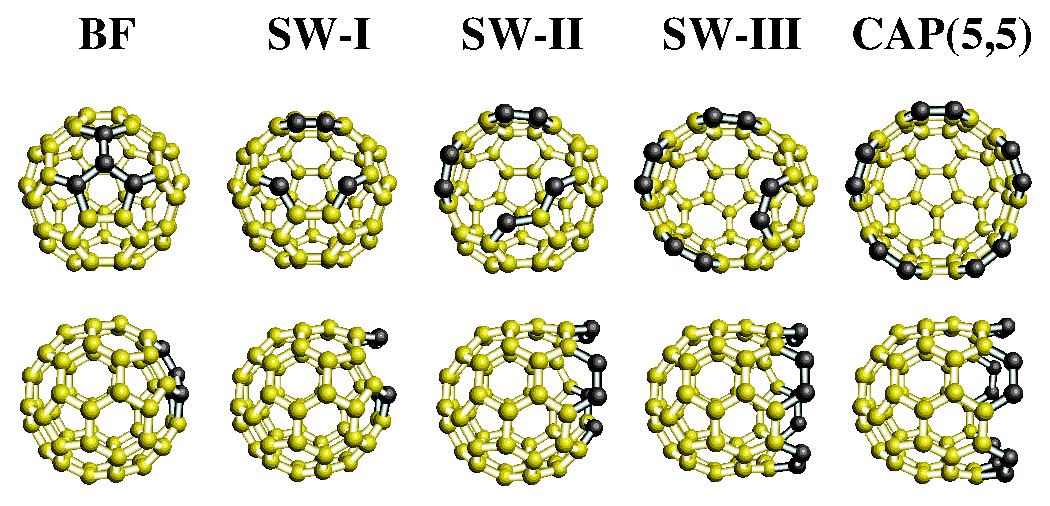
\includegraphics[width=0.5\textwidth]{figures/sample-fig1}
%	\label{fig:sample}
%	\caption{Sample Figure}
%\end{figure}
%
%\section{Answer to RQ2 : Computational simulation predicts causal relationship of exceed motor command in M1 from VL in Parkinson’s disease patient}
%
%\subsection{ The high synchronization (correlated neural activities) in VL but not average firing rate can drive M1’s motor command}
%
%
%Figure .2.1 The high synchronized neural activities during bursting can drive M1 in WT types but not KO, even though the average firing rate if WT and KO are not significantly difference
%
%
%\subsection{  The high synchronization level can be achieved by bursting. The demolishing of bursting in WT neurons result in the absent of synchronization in neuron population}
%
%Figure .2.2 Schematic diagram of how the bursting activity cause high synchronization in neuron population
%
%\subsection{ The Analysis of information transfer from VL to M1 : The information in VL can transfer to M1 when the neuron population in VL are synchronized }
%
%Figure .2.3 the neural information from VL is transferring to M1 only when the neural activities in VL are synchronized.
%
%Figure .2.4 the level of information transfer between VL and M1 is proportionally to the synchronization level in VL
%
%\subsection{ Artificially generated bursting in KO neurons result in high synchronization level of neuron population which can drive M1’s motor command
%}
%Figure .2.5 successfully generated bursting behavior in KO with similar bursting behavior generated by T-Type Calcium channel in WT
%
%Figure .2.6 The artificial bursting behavior in KO result in high level synchronization level of neural population and this high synchronized neural 
%population can drive M1
%
%\subsection{ Artificially activated VL neural population in theta and beta frequencies result in motor command from M1with the same frequency band with what observed in Parkinson’s disease patient.}
%
